\documentclass[10pt,a4paper]{article}
\usepackage[margin=0.68in,headheight=14pt,headsep=12pt,footskip=22pt]{geometry}
\usepackage[T1]{fontenc}
\usepackage{lmodern,microtype}
\usepackage{amsmath,amssymb,graphicx,booktabs,tabularx,array}
\usepackage{xcolor,listings,enumitem,titlesec,fancyhdr,caption,etoolbox}
\usepackage[colorlinks=true,urlcolor=blue!55!black,linkcolor=blue!55!black]{hyperref}

% Add the real repository URL before submission. Do not use the upstream
% simulator repository as the project repository.
\newcommand{\repositoryURL}{https://github.com/nidhish1/rl-optimal-control-project}
% Optional: enter your name, student ID and course here.
\newcommand{\authorDetails}{}

\definecolor{navy}{HTML}{193B56}
\definecolor{pale}{HTML}{F1F5F9}
\definecolor{muted}{HTML}{4B5967}
\setlength{\parindent}{0pt}
\setlength{\parskip}{4pt}
\setlength{\tabcolsep}{5pt}
\renewcommand{\arraystretch}{1.13}
\setlist[itemize]{leftmargin=*,nosep,topsep=2pt}
\titleformat{\section}{\large\bfseries\color{navy}}{\thesection.}{0.45em}{}
\titlespacing*{\section}{0pt}{9pt}{4pt}
\captionsetup{font=small,labelfont=bf,skip=4pt}
\pagestyle{fancy}
\fancyhf{}
\fancyhead[L]{\small\color{muted}DreamNav \;|\; Preliminary project report}
\fancyhead[R]{\small\color{muted}Robotics / Reinforcement Learning}
\fancyfoot[R]{\small\thepage\,/\,2}
\renewcommand{\headrulewidth}{0.3pt}
\fancypagestyle{plain}{\fancyhf{}\fancyfoot[R]{\small\thepage\,/\,2}\renewcommand{\headrulewidth}{0pt}}
\lstdefinestyle{compact}{basicstyle=\ttfamily\fontsize{8.1}{9.8}\selectfont,
  backgroundcolor=\color{pale},frame=single,rulecolor=\color{black!15},
  framesep=5pt,aboveskip=4pt,belowskip=0pt,breaklines=true,
  showstringspaces=false,columns=fullflexible,keepspaces=true,
  keywordstyle=\color{navy}\bfseries,commentstyle=\color{muted}}
\newcolumntype{Y}{>{\raggedright\arraybackslash}X}
\begin{document}
\thispagestyle{plain}
{\LARGE\bfseries\color{navy}DreamNav}\par
{\large World-Model-Based Autonomous Quadcopter Navigation}\par
{\small\color{muted}Preliminary project report}
\ifdefempty{\authorDetails}{}{\par{\small\authorDetails}}

\textbf{Project GitHub repository:}
\ifdefempty{\repositoryURL}
{\textit{Pending creation; the project URL will be added before submission.}}
{\expandafter\url\expandafter{\repositoryURL}}

\section{Project description}
DreamNav investigates whether a drone can navigate using a learned model of the consequences of its actions. A simulated quadcopter must reach three ordered 3D waypoints among static obstacles. A gated recurrent unit (GRU) predicts candidate flight trajectories; model predictive control (MPC) selects a command and replans after receiving new observations. A proximal policy optimization (PPO) policy provides the model-free reinforcement-learning baseline. The objective is a reproducible navigation demonstration and comparison, rather than a new RL algorithm. Hardware deployment, raw-camera perception and motor-level RL are outside the core scope.

\section{Tools and existing code}
\begin{tabularx}{\linewidth}{@{}>{\raggedright\arraybackslash}p{0.25\linewidth}Y@{}}
\toprule
\textbf{Tool / dependency} & \textbf{Role and project-specific work} \\
\midrule
PyBullet + \texttt{gym-pybullet-drones} [1] & Existing Crazyflie CF2X physics and PID stabilization; custom rooms, 32-ray LiDAR, waypoint manager and velocity/yaw command adapter. \\
Python, Gymnasium, PyTorch & Shared environment API; episode logging; GRU training and batched learned-model rollouts. \\
Stable-Baselines3 [2], NumPy, Matplotlib & Existing PPO implementation; numerical processing, comparison plots and video export (ImageIO). \\
\bottomrule
\end{tabularx}
Physics runs at 240\,Hz, PID control at 60\,Hz and navigation at 10\,Hz. The observation $o_t\in\mathbb{R}^{44}$ contains 32 ranges, linear velocity, Euler angles, angular velocity and relative goal position. Four normalized actions command heading-frame planar velocity, vertical velocity and yaw rate. All controllers use the same observation/action interface and physics.

\section{Algorithms and implementation}
\textbf{GRU world model.} An encoder maps $44\!\to\!128\!\to\!64$ features; concatenating four actions gives a 68-dimensional GRU input, with hidden size 128. Residual heads predict the next 44 observation channels and a collision logit. Adam minimizes normalized state/range errors, class-weighted collision binary cross-entropy and a short recursive rollout loss. Training windows stay within episodes and waypoint segments; normalization uses training data only.

\textbf{CEM--MPC.} The cross-entropy method (CEM) samples 128 action sequences, retains 16 elites and refits the sampling distribution for four iterations. The initial horizon is $H=10$ steps (one second). Sequences are scored for goal progress, predicted collision risk, clearance and smoothness, with time/arrival terms. Only the first command is executed. No valid sequence or high immediate risk triggers a zero-velocity command.

\textbf{PPO baseline.} PPO [2,3] trains separate actor/critic MLPs with two 256-unit hidden layers using on-policy rollouts and a clipped policy objective. It maps observations directly to continuous commands. In contrast, the GRU learns dynamics by supervised learning; MPC is an online optimizer, not a trained RL actor.

\begin{minipage}[t]{0.485\linewidth}
\textbf{Pseudocode: one navigation loop}
\begin{lstlisting}[style=compact]
observe o; keep real-history state h
repeat 4 CEM iterations:
  sample 128 bounded action sequences
  copy h for each candidate
  predict 10 steps with the GRU
  score progress, risk and smoothness
  refit mean/std from 16 valid elites
choose best sequence (or zero fallback)
execute its first action through PID
update h using the real observation/action
on goal change: reset h and plan anew
repeat until success, collision or timeout
\end{lstlisting}
\end{minipage}\hfill
\begin{minipage}[t]{0.485\linewidth}
\textbf{Key code excerpts (reformatted)}
\begin{lstlisting}[style=compact,language=Python]
# model.py: recurrent prediction heads
self.gru = nn.GRU(68, 128, batch_first=True)
self.delta = nn.Linear(128, 44)
self.collision = nn.Linear(128, 1)

# planner.py: CEM update after valid scoring
elite_ids = scores.topk(
    min(cfg.elites, valid_count)).indices
elites = actions[elite_ids]
mean = elites.mean(0)
std = elites.std(0, unbiased=False).clamp_min(
    cfg.min_std)
\end{lstlisting}
\end{minipage}

\newpage
\section{Preliminary work completed}
The simulation, collection, GRU--MPC, PPO and evaluation/video pipelines are implemented. Random commands and noisy guidance generated \textbf{200,056 training transitions} in 1,534 episodes; disjoint validation/test sets contain 20,049/20,010 transitions. The GRU trained for 30 epochs with 32-step windows and five-step rollout loss; validation selected epoch 24. PPO used \textbf{200,704 transitions}. Both used one training seed. Collection, validation and compute costs are recorded separately; these budgets do not imply equal total cost.

\begin{center}
\small
\begin{tabular}{@{}lrrrrr@{}}
\toprule
\textbf{Controller} & \textbf{Success} & \textbf{Collisions} & \textbf{Time (s)} & \textbf{Path (m)} & \textbf{Decision (ms)} \\
\midrule
Scripted guidance & 30/30 & 0/30 & 13.81 & 7.03 & 0.052 \\
GRU + CEM--MPC & 30/30 & 0/30 & 8.84 & 7.67 & 12.35 \\
PPO & 30/30 & 0/30 & 8.12 & 8.01 & 0.077 \\
\bottomrule
\end{tabular}
\end{center}
\vspace{-4pt}
{\small\textbf{Table 1.} Same 30 held-out, three-waypoint courses per controller; time is simulated mission duration. Path/time and decision latency are means. Latency excludes rendering and is measured locally.}

\vspace{5pt}
\begin{minipage}[t]{0.47\linewidth}
\vspace{0pt}
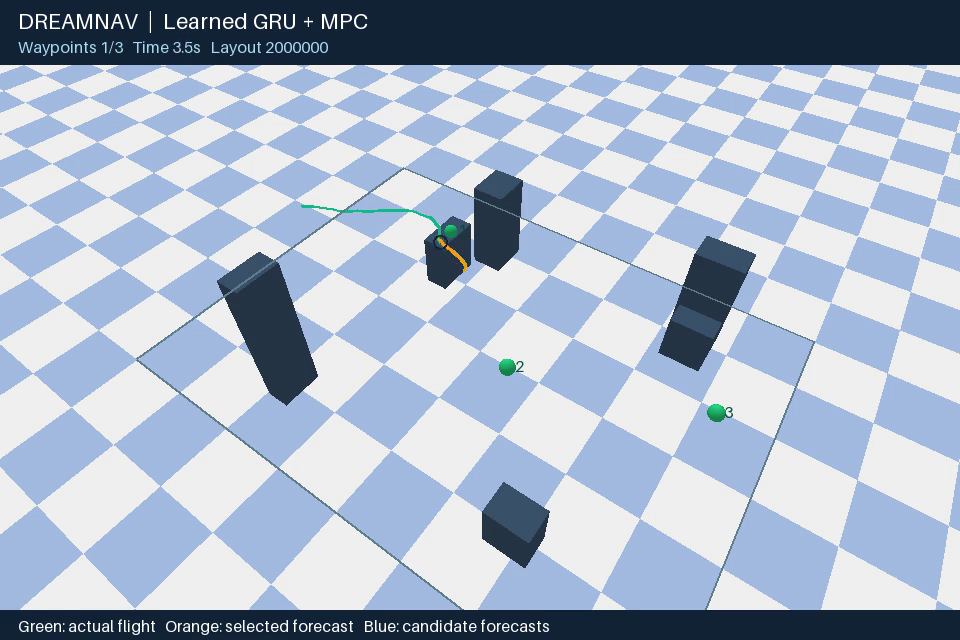
\includegraphics[width=\linewidth]{figures/mpc_demo.png}
\captionof{figure}{Recorded GRU--MPC flight: actual path (green), selected forecast (orange), other candidates (blue) and waypoints (spheres).}
\end{minipage}\hfill
\begin{minipage}[t]{0.50\linewidth}
\vspace{0pt}
\textbf{Prediction and verification.} On the same 256 sampled test windows, 10-step LiDAR RMSE was 0.509\,m versus 0.631\,m for a persistence predictor. One-step collision recall was 88.4\% and precision 40.9\% at threshold 0.5 over 43 positive events in 20,010 transitions. Long-horizon collision prediction remains insufficiently validated.

Automated checks cover flight stability, sensing, seeded resets, collision/timeout handling, sequence boundaries, waypoint changes and recurrent planning state. A complete collection--training--evaluation smoke run and annotated flight videos are available.
\end{minipage}

\textbf{Interpretation and limits.} These initial courses reserve a clear tube along the waypoint route, use a fixed room/start and only modest goal variation. Scripted guidance also succeeds on every course. The results establish that the pipeline functions; they do \emph{not} demonstrate superiority over PPO or reliable navigation in arbitrary obstacle layouts.

\section{Planned work, experiments and expected outcomes}
\begin{tabularx}{\linewidth}{@{}>{\raggedright\arraybackslash}p{0.21\linewidth}Y>{\raggedright\arraybackslash}p{0.27\linewidth}@{}}
\toprule
\textbf{Next stage} & \textbf{Experiment / planned work} & \textbf{Measurement / expected insight} \\
\midrule
Harder navigation & Add blocked direct paths, narrow passages and varied starts/room widths; test frozen models on new layouts. & Success, collisions and efficiency; reveal limits hidden by easy courses. \\
Prediction and planning & Add successful model-based flights to training replay; inspect 1/5/10/20-step errors; vary $H\in\{5,10,20\}$ and candidate count. & Forecast drift, collision calibration and latency; test the horizon--compute trade-off. \\
Long missions and fairness & Compare 1/3/5/8 waypoints; repeat training with three seeds and at least 30 held-out episodes per setting. & Mission success, checkpoints reached, mean/dispersion; assess accumulated errors. \\
Optional extension & Replace GRU with a causal Transformer; match data/planner settings and study occlusion or sensor dropout. & Test whether longer memory helps prediction and navigation; not yet implemented. \\
\bottomrule
\end{tabularx}
\textbf{Expected deliverables.} Reproducible repository, checkpoints, comparison plots, annotated demo and final report quantifying accuracy, efficiency and planning cost. Outperforming PPO is a hypothesis, not a guaranteed result.

\vspace{3pt}
{\footnotesize\color{muted}
\textbf{References and evidence.}
[1] Panerati et al., \href{https://arxiv.org/abs/2103.02142}{\emph{Learning to Fly}}, IROS 2021; \href{https://github.com/learnsyslab/gym-pybullet-drones}{simulator code}.
[2] \href{https://stable-baselines3.readthedocs.io/en/master/modules/ppo.html}{Stable-Baselines3 PPO documentation}.
[3] Schulman et al., \href{https://arxiv.org/abs/1707.06347}{\emph{Proximal Policy Optimization Algorithms}}, 2017.
Local evidence: \texttt{runs/evaluation/summary.json}, \texttt{runs/forecasts/forecast.json}, training manifests and source modules in \texttt{dreamnav/}.}
\end{document}
